\section{OSI Referenzmodell}
    \subsubsection{Schichten, Protokolle und Dienste}
    \begin{definition}{Systeme}
        Offene Systeme (im Gegensatz zu proprietären Systemen) basieren auf öffentlich verfügbaren Standards für Schnittstellen und Protokolle
    \end{definition}

    \begin{definition}{Dienst}
        sendet und empfängt bestätigte und unbestätigte Daten.
    \end{definition}
    \begin{highlight}{Klassifizierung von Diensten}
    \begin{center}
        \begin{minipage}{0.46\linewidth}
                \tcbsubtitle{Verbindungsorientiert}
                    \begin{itemize}
                        \item Verbindungsaufbau nötig
                        \item Informationen vom Empfänger - Optionen aushandeln
                        \item Reihenfolge der Daten bleibt erhalten
                    \end{itemize}
                \tcbsubtitle{Verbindungslos}
                \begin{itemize}
                    \item Jederzeit (send and forget)
                    \item Ziel muss nicht bereit sein
                    \item einfacher umzusetzen
                \end{itemize}
        \end{minipage}
        \hfill\vline\hfill
        \begin{minipage}{0.47\linewidth}
            \tcbsubtitle{Zuverlässig}
                \begin{itemize}
                    \item Kein Datenverlust
                    \item Sicherung durch Fehler-Erkennung/-Korrektur
                    \item Text-Nachrichten
                \end{itemize}
            \tcbsubtitle{Unzuverlässig}
            \begin{itemize}
                \item Möglicher Datenverlust
                \item Keine Sicherung
                \item Streaming
            \end{itemize}
        \end{minipage}
    \end{center}
\end{highlight}

\begin{definition}{Schicht}
    hat die Aufgabe der darüberliegenden Schicht bestimmte Dienste zur Verfügung zu stellen. Die Schichten benötigen kein Wissen über die Realisierung der darunterliegenden Schicht.
\end{definition}

\begin{definition}{Protokoll}
     eine Sammlung von Nachrichten, Nachrichtenformaten und Regeln zu deren Austausch.\\
     In der Technik ist ein Kommunikationsprotokoll eine Vereinbarung, die festlegt wie eine Datenübertragung zwischen Kommunikationspartnern abläuft.
\end{definition}

\columnbreak

\subsubsection{Datenübertragung und Schichtenmodell}

\begin{concept}{OSI Modell}
    \begin{itemize}
        \item Referenzmodell, beschreibt Kommunikation zwischen räumlich entfernten Kommunikationspartnern
        \begin{itemize}
            \item 7 Schichten (unabhängige Teilfunktionen)
            \item Eine Schicht erfüllt, mit Hilfe der untergeordneten Schichten, bestimmte Aufgaben und bietet der übergeordneten Schicht über eine definierte Schnittstelle einen definierten Dienst an
            \item Gleiche Schichten in verschiedenen Systemen kommunizieren nach den Regeln eines standardisierten Protokolls
        \end{itemize}
        \item Die Kommunikation erfolgt logisch zwischen Protokollimplementierungen auf gleicher Schicht (Kommunikationsbeziehung), physikalisch wandern die Daten beim Sender im Stack «nach unten», werden über ein Medium übertragen, und wandern beim Empfänger wieder «nach oben»
    \end{itemize}
\end{concept}

\begin{definition}{OSI Layers}
    \begin{itemize}
        \item Anwendungsschichten 5-7
        \begin{itemize}
            \item Lösen allgemeine Aufgaben
        \end{itemize}
        \item Transportschichten
        \begin{itemize}
            \item Teil des Betriebssystems und Treiber
            \item «Socket»-Schnittstelle für eigene Anwendungsprotokolle
        \end{itemize}
    \end{itemize}
\end{definition}

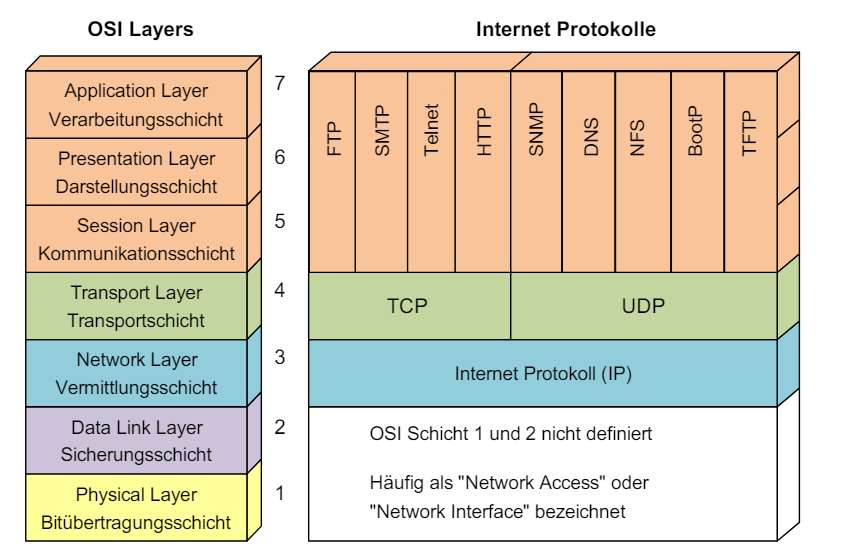
\includegraphics[width=0.9\linewidth]{images/images/OSI_Modell.png}
\includegraphics[width=0.8\linewidth]{images/images/Datenübertragung_Schichtenmodell.png}




 
    
 